\documentclass{article}
\usepackage[x11names, rgb]{xcolor}
\usepackage[utf8]{inputenc}
\usepackage{tikz}
\usetikzlibrary{snakes,arrows,shapes}
\usepackage{amsmath}
%
%

%

%

\begin{document}
\pagestyle{empty}
%
%
%

\enlargethispage{100cm}

\Large
% Start of code
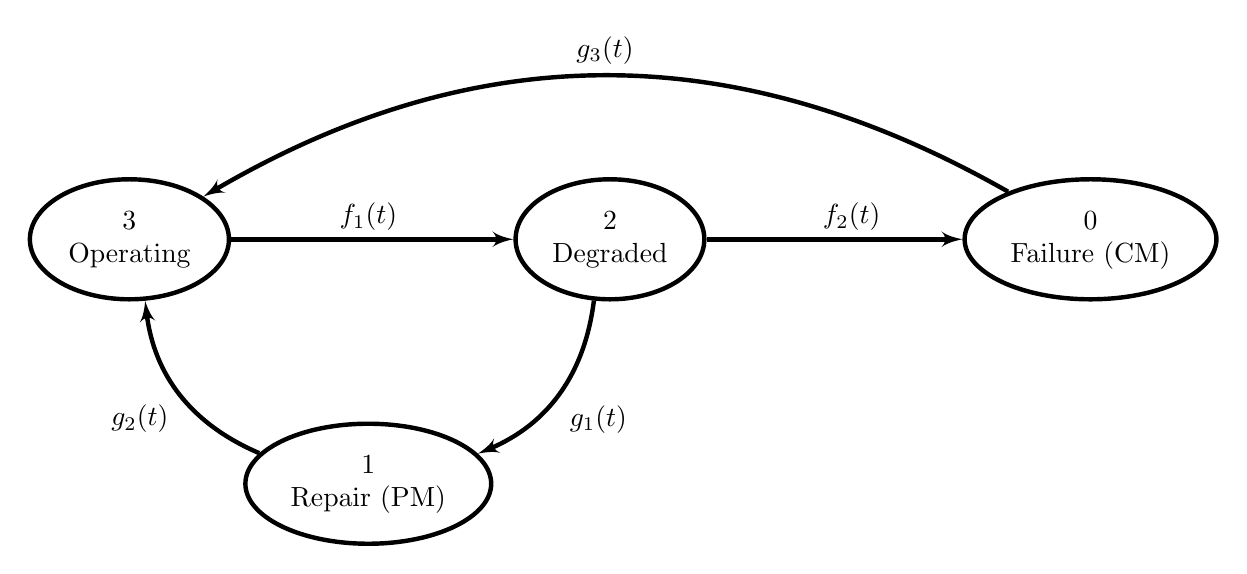
\begin{tikzpicture}[>=latex',line join=bevel,]
%%
\node (1) at (123.31bp,18bp) [draw,ellipse,ultra thick] {$\begin{matrix}1 \\ \text{Repair (PM)}\end{matrix}$};
  \node (0) at (383.31bp,106bp) [draw,ellipse,ultra thick] {$\begin{matrix}0 \\ \text{Failure (CM)}\end{matrix}$};
  \node (3) at (37.314bp,106bp) [draw,ellipse,ultra thick] {$\begin{matrix}3 \\ \text{Operating}\end{matrix}$};
  \node (2) at (210.31bp,106bp) [draw,ellipse,ultra thick] {$\begin{matrix}2 \\ \text{Degraded}\end{matrix}$};
  \draw [->,ultra thick] (2) to[bend left] node[auto] {$g_1(t)$} (1);
  \draw [->,ultra thick] (0) to[bend right] node[above] {$g_3(t)$} (3);
  \draw [->,ultra thick] (2) ..controls (266.59bp,106bp) and (313.4bp,106bp)  .. (0);
  \definecolor{strokecol}{rgb}{0.0,0.0,0.0};
  \pgfsetstrokecolor{strokecol}
  \draw (297.31bp,114bp) node {$f_2(t)$};
  \draw [->,ultra thick] (3) ..controls (93.586bp,106bp) and (140.4bp,106bp)  .. (2);
  \draw (123.31bp,114bp) node {$f_1(t)$};
  \draw [->,ultra thick] (1) to[bend left] node[auto] {$g_2(t)$} (3);
%
\end{tikzpicture}
% End of code

%
\end{document}
%



